% !TEX root = ./main.tex
\documentclass[a4paper]{article}
% Course language: use [english] or [german].
\usepackage[german]{ajnotes}
\title{\textbf{Mikroökonomie — Budget}}
\begin{document}
    \maketitle
    % Attach the given problem sheet: drop it in this folder as sheet.pdf and
    % un-comment the next line (pdfpages is already loaded by the preamble).
    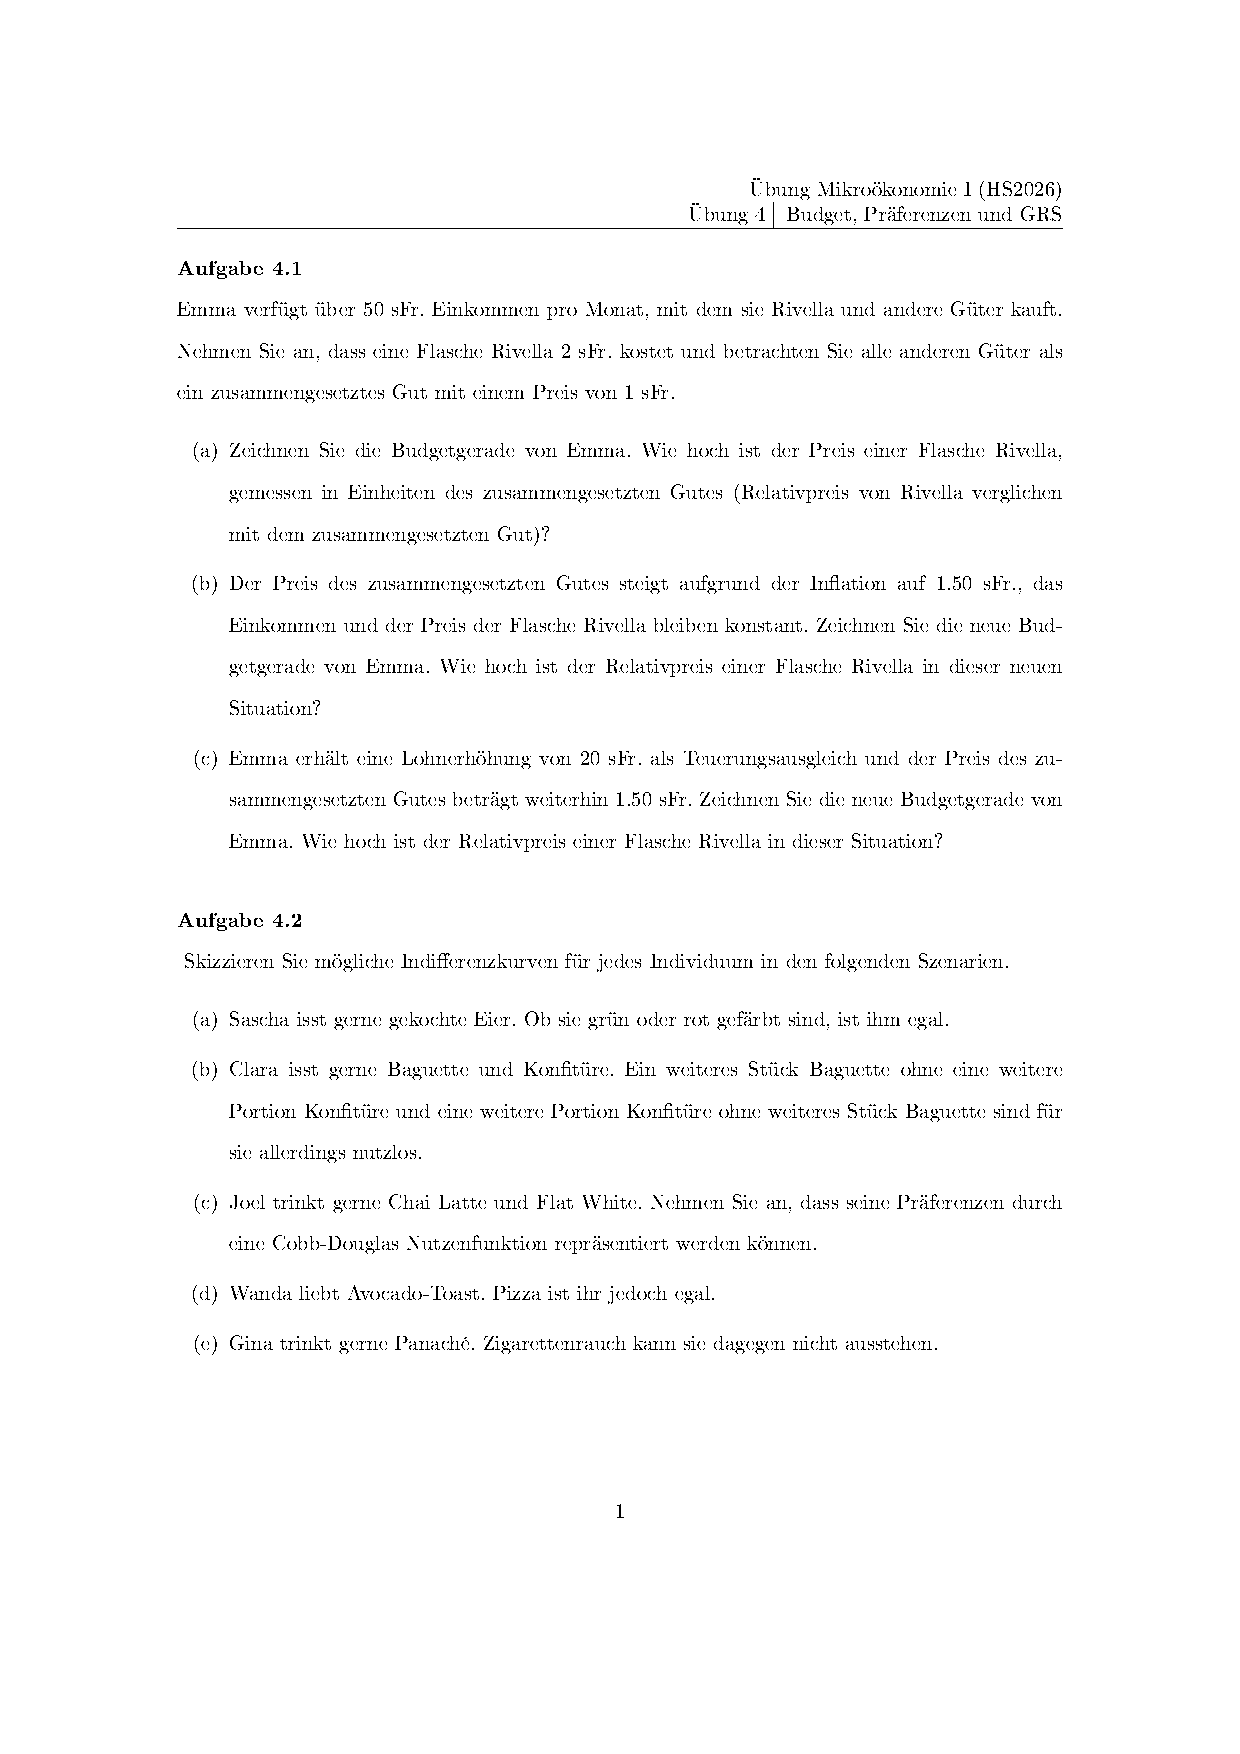
\includepdf[pages=-]{sheet.pdf}
    \exercise{4.1}
        \subexercise{a,b,c}
        \begin{itemize}
            \item  a- Relativ preis rivela = 2x Zusammengesetzt
                
                \item b - Relativ preis ist 2/1.5 = 1.33x Zusammengesetzt
                
            \item  c - immer noch 1.33
                
        \end{itemize}
        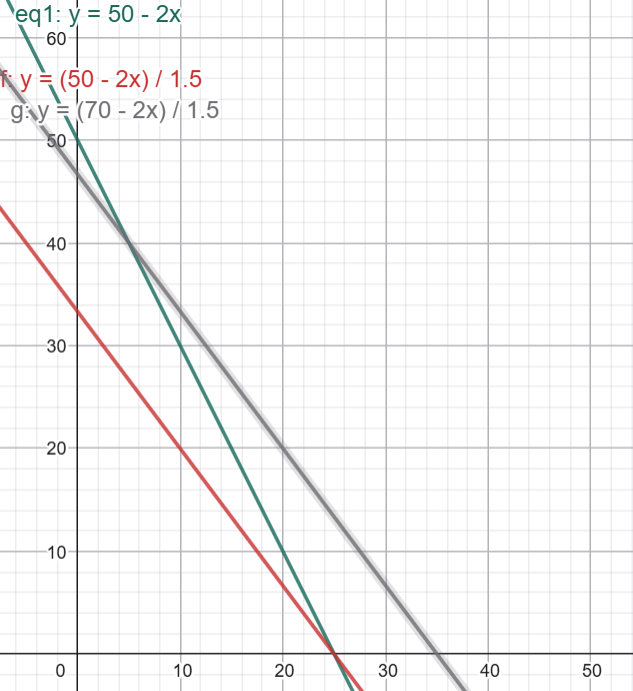
\includegraphics[width=\textwidth,height=0.7\textheight,keepaspectratio]{figures/41_Funktionen.png}

\pagebreak  
    \exercise{4.2}
        \subexercise{a}
        Achsen sind Mengen Grüne (X) und Rote Eier (Y). Linear weil Nutzen nicht von der Aufteilung Grün/Rot abhängt sondern nur von der Summe der Mengen. Nicht Konvex weil extreme Allokationen (40, 0) und (0,40) vorhanden.
        \subexercise{b}
        Nicht gelöst\dots
        \subexercise{c}
        Cobb-Douglas, Konvex weil immer beide Güter immer vorhanden, keine Nullpunkte. 
        \subexercise{d}
        Nutzen nur von der Menge Y abhängig daher waagrecht
        \subexercise{e}
        Linear weil Nutzen von der Summe aus beiden Güter besteht, wobei Rauch(x) eine negative wirkung hat. \break
    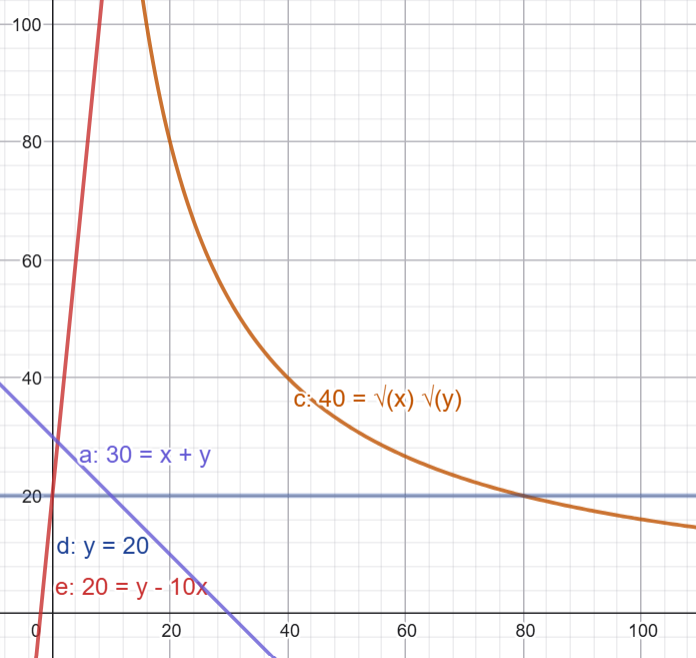
\includegraphics[width=\textwidth,height=0.7\textheight,keepaspectratio]{figures/42_Kurven.png}
    \pagebreak

    \exercise{4.3}
    \subexercise{a}
    \begin{equation}
        U'(f) = 2S 
    \end{equation}
    \begin{equation}
        U'(S) = 2F
    \end{equation}
    \begin{equation}
        GRS  = \frac{U'(S)}{U'(F)} = \frac{2S}{2F} = \frac{S}{F}
    \end{equation}

    \subexercise{b}
    \begin{equation}
        F = \frac{U}{2S} \rightarrow F = \frac{100}{2*2} = 25
    \end{equation}
    \begin{equation}
        GRS = \frac{2}{25} 
    \end{equation}  

    
\end{document}
